\subsubsection{Stochastinis gradientinis nusileidimas}
\label{subsubsec:paklaidos_priklausomybe_stochastinis_gradientinis_nusileidimas}

Naudojant stochastinį gradientinį nusileidimą su tuo pačiu mokymosi greičiu, paklaida mažėja greičiau nei paketinio metodo atveju (žr.~\ref{fig:error_sgd} pav.). Galutinė mokymo paklaida – $0{,}0189$, validavimo – $0{,}0103$. Stochastinis metodas pasiekia mažesnes paklaidas, nes svoriai atnaujinami po kiekvieno pavyzdžio.

\begin{figure}[H]
    \centering
    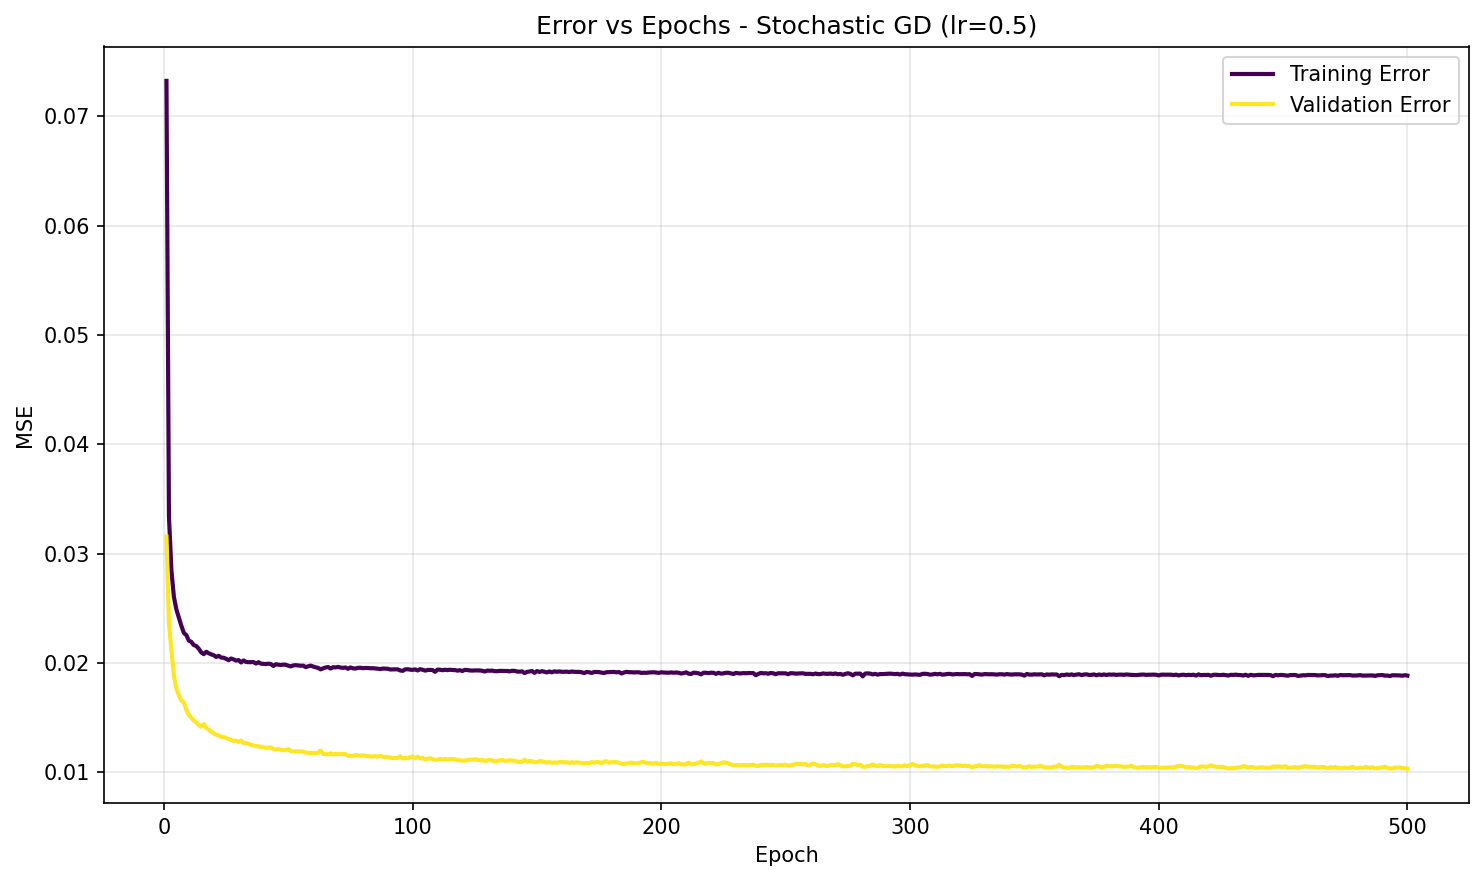
\includegraphics[width=0.85\linewidth]{2Lab/visualizations/error_sgd.png}
    \caption{Paklaidos priklausomybė nuo epochų (stochastinis GN, $\eta = 0{,}5$)}
    \label{fig:error_sgd}
\end{figure}